\chapter{Data and Exploratory Data Analysis}

\section{MuSiQue}
% Source, rationale, characteristics, fields, and limitations.

\section{Exploratory Data Analysis}

\section{Problems Identified}
\label{sec:problems}

The probes need two classes of comparable size: episodes where the Solver
adopts the Critic's answer and episodes where it keeps its own. The original
design produced almost none of the second kind. This section describes the
problem, the changes we tried, and why we settled on one feedback condition
and added synthetic questions.

\subsection{Too Few Retention Cases}

With free-form feedback, where the Solver revised its answer after reading
the Critic's full review, the Solver followed the Critic almost every time
they disagreed. Under the rule-based labels, 91.7\% of the 4,177 Adoption and
Retention episodes in the training partition were Adoption, and a sample
labeled by Claude gave 97.3\%. The negative-class audit
(Section~\ref{sec:negative-audit}) found only 347 eligible Retention episodes
against 3,830 eligible adoptions in training, and showed that many labeled
negatives were not genuine rejections. A probe trained on these labels would
mostly learn the majority class.

\subsection{What We Tried}

Table~\ref{tab:balance-attempts} lists the changes in the order we made them.
Each one targeted a specific cause of the imbalance.

\begin{table}[htbp]
    \centering
    \caption{Changes tried to obtain enough Retention episodes. Shares are
    of the Adoption and Retention episodes in each run.}
    \label{tab:balance-attempts}
    \small
    \begin{tabular}{p{3.0cm}p{3.6cm}p{4.6cm}p{3.2cm}}
        \toprule
        Change & Why & Result & Decision \tabularnewline
        \midrule
        \raggedright Gemma as its own Critic (200 questions)
            & \raggedright The proposal's design
            & \raggedright The Critic repeated A1 in 179 of 183 reviews.
            & \raggedright Use Qwen as the Critic
              (Section~\ref{sec:two-models}). \tabularnewline
        \raggedright Free-form feedback from Qwen (MuSiQue)
            & \raggedright Independent feedback should create real
              disagreement
            & \raggedright Disagreement appeared, but 91.7\% of the binary
              episodes were Adoption.
            & \raggedright Change how the feedback is shown. \tabularnewline
        \raggedright Presentation pilot (80 questions, 8 formats)
            & \raggedright Test whether the format of the feedback drives
              adoption
            & \raggedright Retention was 10\% with feedback text and 47--72\%
              when A1 and C1 were shown as two candidates.
            & \raggedright Adopt the candidate presentation. \tabularnewline
        \raggedright Candidate presentation (MuSiQue, 22,355 episodes)
            & \raggedright Apply the best format to the full dataset
            & \raggedright Adoption fell to 54.8\% of 10,644 binary episodes;
              listing the Critic first raised it by 4--9 points.
            & \raggedright Keep it; randomize and balance the order.
              \tabularnewline
        \raggedright Synthetic questions
            & \raggedright More and cleaner disagreement than MuSiQue can
              supply
            & \raggedright Section~\ref{sec:synthetic-data}.
            & \raggedright Combine with MuSiQue. \tabularnewline
        \bottomrule
    \end{tabular}
\end{table}
% Sources: notebooks/collection/experiment_analysis.ipynb (rows 1-3);
% results/claude_validation/adoption_conditions_80q_opus5_summary/summary.json
% (presentation pilot); PR #170 and reports/tables/candidate_order_balance/ (order).

The decisive change was how the feedback was shown, not who gave it. When the
Solver read a critique, it almost always deferred. When it chose between two
labeled answers, its own and the reviewer's, it kept its own answer about half
the time. The candidate presentation is described in
Section~\ref{sec:forward-pass}.

The candidate format introduced a new problem: the order of the two answers
affected the choice. On the MuSiQue collection, listing the Critic's answer
first raised the Adoption share from 51.9\% to 57.8\%, and the gap appeared in
every partition (Figure~\ref{fig:order}a). We therefore assign each question
one of the two orders at random, balanced within each hop type, and record it,
so that order can be checked as a confound in every analysis
(Section~\ref{sec:results-labels}).

The same data show a second pattern (Figure~\ref{fig:order}b). We call a
correction \emph{right} when A1 is wrong and the Critic's recommendation is
right, and \emph{wrong} when A1 is right and the recommendation is wrong.
Correctness is the collection's exact match against the gold answer and its
aliases, after normalizing case, punctuation and articles. The Solver adopted
wrong corrections more often than right ones: 56.6\% ($n = 745$) and 60.6\%
($n = 769$), against 40.2\% ($n = 955$) and 43.6\% ($n = 928$), with A1 and
with the Critic listed first. This is an association observed in the 3,397
binary episodes where exactly one of the two answers was right, out of
10,644. It does not show that wrong feedback causes adoption: the Critic's
correctness was not controlled, which is what the dropped controlled
conditions would have done. The exact-match check also counts some correct
answers written as full sentences as wrong. Even so, adoption is not a
reliable sign that the Solver recognizes good feedback, which is why the
labels describe behavior rather than correctness
(Section~\ref{sec:problem-definition}).
% Source: reports/tables/candidate_order_balance/candidate_order_correctness.csv
% (rows "all"; PR #153 rule-based labels, MuSiQue candidate collection).

\begin{figure}[htbp]
    \centering
    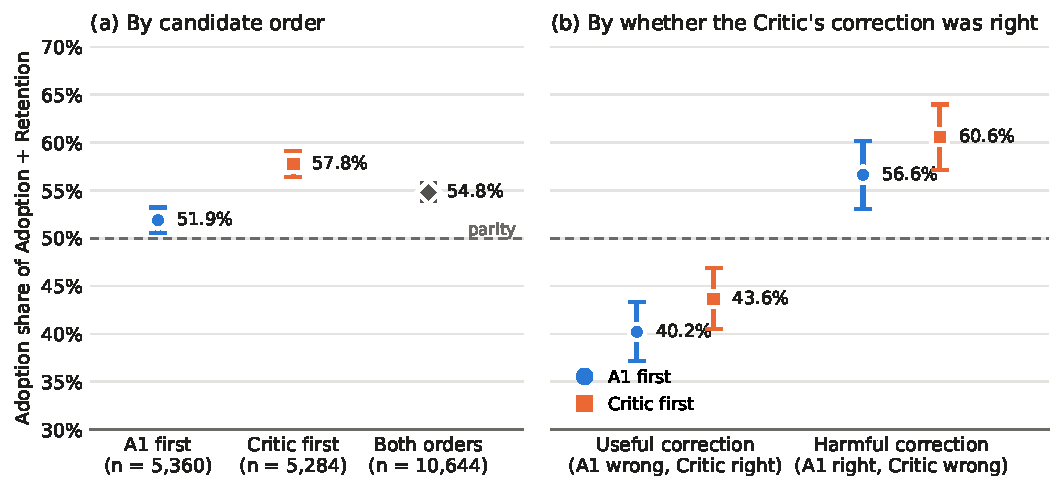
\includegraphics[width=0.8\textwidth]{candidate_order_adoption.pdf}
    \caption{Adoption share of the Adoption and Retention episodes, with 95\%
    Wilson intervals (MuSiQue candidate collection, rule-based labels).
    (a)~By candidate order: listing the Critic's answer first raises
    adoption. (b)~By whether the Critic's correction was right: the Solver
    adopts wrong corrections more often than right ones, in both orders.}
    \label{fig:order}
\end{figure}

\subsection{How Many Feedback Conditions}

The proposal planned three feedback conditions: natural feedback, a Critic
given the correct answer, and a Critic given a plausible wrong answer. The two
controlled conditions were meant to separate general deference from
recognizing good feedback. In the first 200-question run they did not work as
intended: the Critic's wording revealed that an answer had been supplied to
it, and the supplied wrong answers often did not fit the question. Natural
feedback from Qwen already produced the variation we needed, with the Solver
adopting, keeping or changing its answer, so we narrowed the study to the
natural condition. The controlled conditions remain implemented in the code.
Dr.~Jafari confirmed that they were not required (team reply to Instructor
Review~\#7, 7~November 2026). The cost is that the study cannot fully separate
deference from discrimination, a limitation we return to in the discussion.

\subsection{Why Synthetic Data}

The candidate presentation solved the balance problem but not the size
problem. MuSiQue's answerable training and validation questions yielded only
10,644 Adoption and Retention episodes, and part of MuSiQue's disagreement
comes from defects in the dataset rather than from the Solver: garbled
composed questions, gold answers that do not fit the question, and paragraphs
that do not state the relation they are cited for. In a 100-question control
sample the Critic refused to answer 17\% of MuSiQue questions. To obtain more
and cleaner disagreement, we generated synthetic questions in the MuSiQue
format.

\section{Synthetic Data}
\label{sec:synthetic-data}

The synthetic questions had one job: to add Adoption and Retention episodes
that come from real reasoning disagreements, ideally a wrong first answer that
the Critic can correct, without MuSiQue's defects. The generation procedure is
described in Section~\ref{sec:synthetic-generation}. This section covers what
the questions had to look like and how we checked that they served their
purpose.

\subsection{Required Characteristics}

Each synthetic question had to meet the following requirements, all enforced
by the generator's prompt or by automatic checks before a question was
accepted:
\begin{itemize}
    \item \textbf{The MuSiQue format}, so the same pipeline, prompts and
    labels apply unchanged: a question, its paragraphs, an answer with
    aliases, and a step-by-step decomposition.
    \item \textbf{The same six hop types} (2hop, 3hop1, 3hop2, 4hop1, 4hop2,
    4hop3). Each step expresses one relation supported by one paragraph, and
    the question needs every supporting paragraph without revealing the
    intermediate answers.
    \item \textbf{The paragraphs are the only ground truth.} Facts need not be
    true in the real world, but the question, answers, supporting paragraphs
    and distractors must be consistent with each other.
    \item \textbf{Related distractor paragraphs} that neither contradict the
    evidence nor answer the question.
    \item \textbf{Short answers} (entities, dates or numbers), so that both
    the labels and correctness can be judged.
    \item \textbf{No overlap with MuSiQue}: every question is validated for
    structure and checked against MuSiQue's training and validation questions
    for duplicates.
\end{itemize}

\subsection{Pilot: Do Synthetic Questions Produce Useful Disagreement?}

Before adding synthetic questions to the training data, we collected 100 of
them with the same models, presentation and decoding settings as MuSiQue,
next to 100 MuSiQue questions matched by hop type
(Figure~\ref{fig:synthetic-pilot}). The first synthetic set did not behave
like MuSiQue: only 16 of 100 episodes were Adoption or Retention, against 56
of 100 for MuSiQue. The difference arose before the feedback. The Solver
answered 78\% of the synthetic questions correctly on its first attempt and
the Critic 90\%, so the two usually agreed on the right answer.

\begin{figure}[htbp]
    \centering
    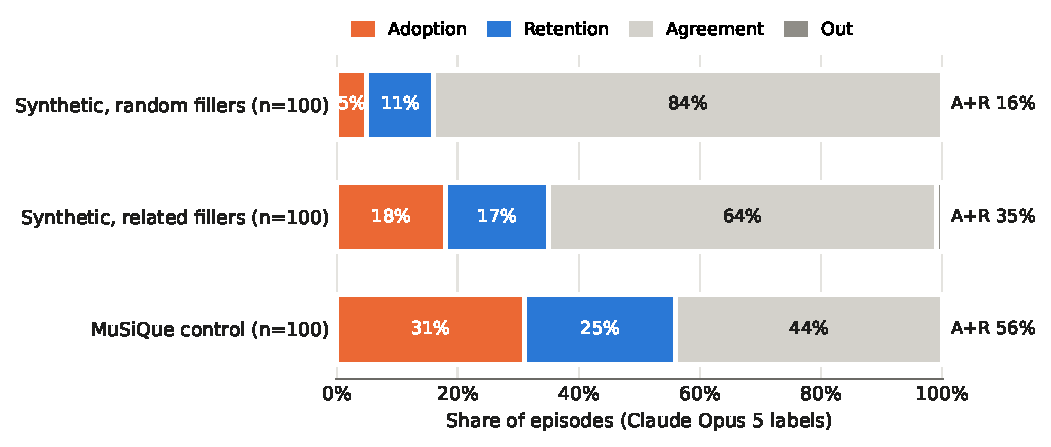
\includegraphics[width=0.85\textwidth]{synthetic_vs_musique_behavior.pdf}
    \caption{Behavior labels for 100 synthetic questions with random filler
    paragraphs, the same questions with related fillers, and 100 MuSiQue
    questions matched by hop type (labels by Claude Opus~5).}
    \label{fig:synthetic-pilot}
\end{figure}

Two findings shaped how we used the synthetic data. First, MuSiQue's rate is
the wrong target. Most synthetic disagreements were the clean case, a wrong
first answer that the Critic corrected (12 of 16), whereas more than half of
MuSiQue's involved two wrong answers (32 of 56). What matters is enough clean
disagreement, not matching MuSiQue. Second, the filler paragraphs, drawn at
random from MuSiQue, rarely competed with the evidence. Replacing only the
fillers with MuSiQue paragraphs similar to the question raised the Adoption
and Retention share from 16\% to 35\% on the same questions (exact McNemar
test, $p < 0.001$), mainly by making the Solver's first answer wrong more
often (A1 accuracy fell from 78\% to 65\%). A replication on 100 new questions
moved in the same direction but was inconclusive: from 18\% to 27\%
(+9 points, 95\% CI $-0.5$ to $+18.5$; $p = 0.093$).
% TODO (Raye): state in Section 6.3 which filler paragraphs the final
% synthetic set (synthetic-final-001) uses.
% Sources: reports/tables/synthetic_pilot/; results/experiments/holdout100_filler_paired/summary.json

\subsection{Synthetic Questions in the Final Dataset}

The final collection contains 79,036 synthetic episodes, spread almost evenly
over the six hop types (12,928--13,303 each). MuSiQue contributes 22,132
episodes, 70\% of them two-hop. The synthetic questions are therefore harder
in structure, with far more three- and four-hop questions, while individual
questions are cleaner. This difference in distribution is a threat to
validity that we examine in the discussion, and Section~\ref{sec:results-labels}
compares the labels of the two sources.

\section{Final Dataset}
% Episode counts, conditions, class balance, splits, and question-family
% grouping used to prevent leakage.
